\providecommand{\tightlist}{\setlength{\itemsep}{0pt}\setlength{\parskip}{0pt}}

\documentclass[a4paper]{jsarticle}
%\usepackage{amsmath,amssymb}
\usepackage{bm}
\usepackage[dvipdfmx]{graphicx}

\usepackage{longtable,booktabs}
\interfootnotelinepenalty=10000


\usepackage[truedimen,mag=1200,top=30truemm,bottom=20truemm,left=25truemm,right=25truemm]{geometry}



\usepackage{ascmac}
\usepackage[dvipdfmx]{hyperref}

\title{付録資料}
\author{松浦知也}



\begin{document}

\maketitle

本付録資料は添付するデータDVDの内容と、再展示のための手順書から成る。

\section{添付データDVDディレクトリ構成}\label{ux6dfbux4ed8ux30c7ux30fcux30bfdvdux30c7ux30a3ux30ecux30afux30c8ux30eaux69cbux6210}

\begin{itemize}
\tightlist
\item
  archive\_data
  記録写真、動画、展示の告知やパンフレットのデータや制作時のメモなど

  \begin{itemize}
  \tightlist
  \item
    documents パンフレットやチラシのデータなど
  \item
    exhibition\_plan 展示プラン、舞台図
  \item
    memo\_nagurigaki 展示に至るまでに作られたメモ書きの寄せ集め
  \item
    photo 製作途中の記録写真、動画など
  \item
    photo\_noguchi 本番の記録写真
  \item
    movie 本作の記録動画(添付記録映像DVDと同じもの)と前作《Acoustic
    Delay (⇔) Memory》の記録動画
  \end{itemize}
\item
  program\_source 実際に展示に使われたスクリプトなどをまとめたフォルダ

  \begin{itemize}
  \tightlist
  \item
    pc1
  \item
    pc2
  \item
    pc3
  \item
    pc4\_5
  \end{itemize}
\item
  readme この文章のソースフォルダ。

  \begin{itemize}
  \tightlist
  \item
    Makefile makeを使用しpdf出力が可能。要pandoc+platex
  \item
    md/readme.md この文章のソースファイル。
  \item
    tex pdf出力用のtexフォルダ。
  \item
    pdf/readme.pdf 本資料のPDFファイル。
  \end{itemize}
\item
  signal\_svg
  Faustでの信号処理のブロックダイヤグラム画像。process.svgをWebブラウザで開くとダイヤグラムが表示される。

  \begin{itemize}
  \tightlist
  \item
    16qam\_2speaker-svg(PC1,2)
  \item
    16qam\_mobiledecoder-svg(PC2,3)
  \end{itemize}
\end{itemize}

\section{《送れ|遅れ /
post|past》展示手順}\label{ux9001ux308cux9045ux308c-postpastux5c55ux793aux624bux9806}

\subsection{展示構成}\label{ux5c55ux793aux69cbux6210}

\subsubsection{展示会場図}\label{ux5c55ux793aux4f1aux5834ux56f3}

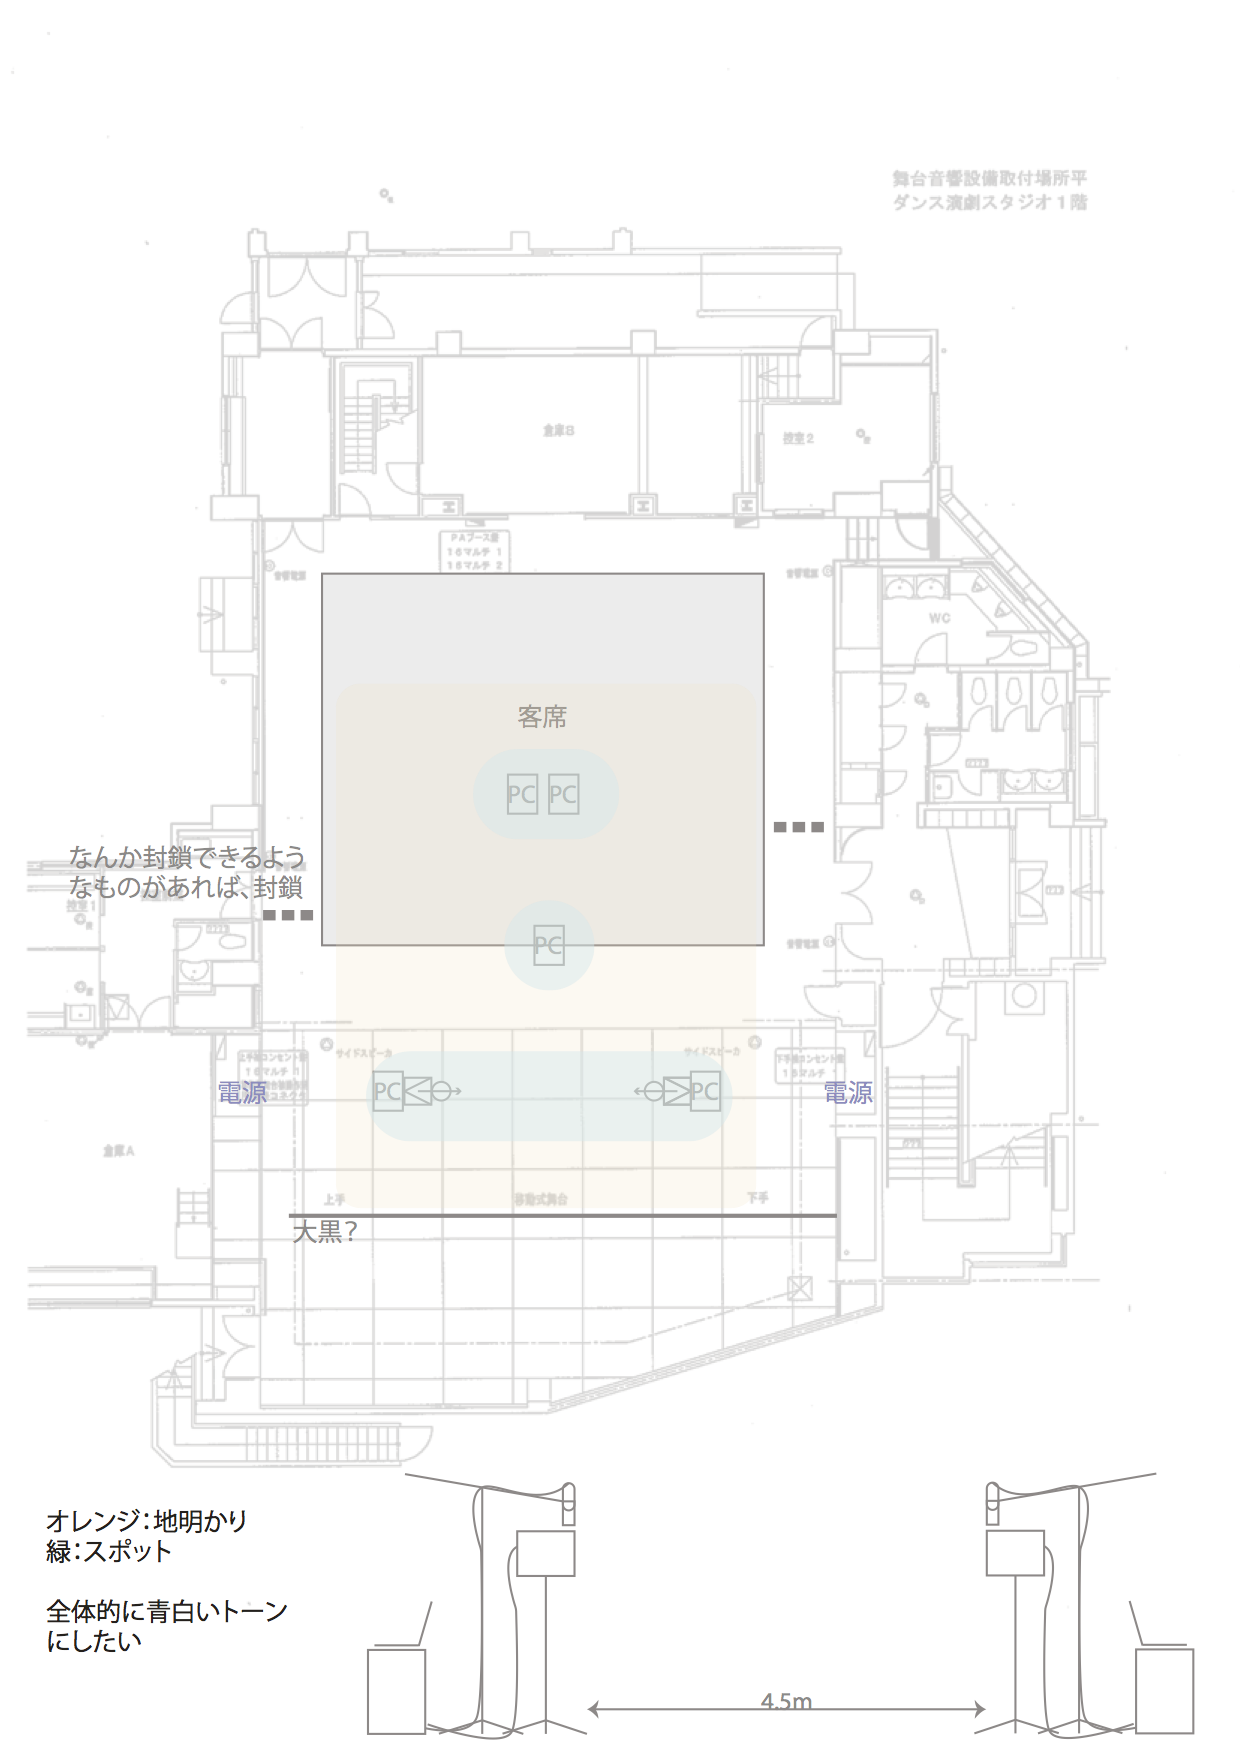
\includegraphics[width=1.00000\textwidth]{../archive_data/exhibition_plan/161030exhibition_plan_light.png}~

\subsection{前準備}\label{ux524dux6e96ux5099}

添付資料内program\_sourceフォルダを各PCのデスクトップにコピーする。

\subsection{PC1/2}\label{pc12}

\subsubsection{使用機材}\label{ux4f7fux7528ux6a5fux6750}

\begin{itemize}
\tightlist
\item
  Macbook Pro
\item
  オーディオインターフェース

  \begin{itemize}
  \tightlist
  \item
    中間発表展示時にはPC1にSteinberg UR28M、PC2にSteinberg
    MR816Xを用いた。比較的低レイテンシなものが望ましいが基本的にはファンタム電源の入る1in1out以上の入出力のあるものならなんでもよい。
  \end{itemize}
\item
  スピーカー

  \begin{itemize}
  \tightlist
  \item
    中間発表時はマイクスタンド設置のできるEVE Audio SC204を使用した。
  \end{itemize}
\item
  マイク

  \begin{itemize}
  \tightlist
  \item
    中間発表時はAKG
    P420を双指向性のモードでパッド、ローカット無しで用いた。
  \end{itemize}
\end{itemize}

\subsubsection{ソフトウェア構成}\label{ux30bdux30d5ux30c8ux30a6ux30a7ux30a2ux69cbux6210}

2016年11月のソフトウェア構成

\begin{itemize}
\tightlist
\item
  OS

  \begin{itemize}
  \tightlist
  \item
    Mac OS X 10.8〜10.12
  \end{itemize}
\item
  ソフトウェア

  \begin{itemize}
  \tightlist
  \item
    Cycling'74 Max v.7.3.1(PC2は都合上OS10.6を利用したため、Max6
    Runtimeを用いた。)
  \item
    faustgen\textasciitilde{} v1.10
  \end{itemize}
\item
  (以下は書き込み機能のPC2のみ)

  \begin{itemize}
  \tightlist
  \item
    Node.js v.5.3.1
  \item
    Google Chrome v.54
  \item
    Safari v.9.1
  \end{itemize}
\end{itemize}

\subsubsection{起動手順}\label{ux8d77ux52d5ux624bux9806}

\paragraph{PC1,2共通(1)}\label{pc12ux5171ux901a1}

\begin{enumerate}
\def\labelenumi{\arabic{enumi}.}
\tightlist
\item
  PCを起動する。
\item
  オーディオインターフェースの電源を入れる。マイクのゲインを最小にし、ファンタム電源を入れる。
\item
  スピーカーの電源を入れる(パッシブタイプを使う場合、パワーアンプの電源を入れる)。ボリュームは最小にしておく。
\end{enumerate}

\paragraph{PC1}\label{pc1}

\begin{enumerate}
\def\labelenumi{\arabic{enumi}.}
\tightlist
\item
  pc1/16qam\_2speaker.maxpatを起動する。
\end{enumerate}

\paragraph{PC2}\label{pc2}

\begin{enumerate}
\def\labelenumi{\arabic{enumi}.}
\tightlist
\item
  Google Chromeを起動する。Google
  Docsで任意の書類を一つ作り、公開範囲をリンクを知っている全員に設定する。
\item
  pc2/16qam\_2speaker.maxpatを起動する。
\item
  Safariを起動する。
\item
  Safariのウィンドウが画面左半分、Google
  Chromeのウィンドウが右半分になるようにウィンドウの大きさを調整する。
\item
  pc2/server\_start.commandを起動する。ターミナルが立ち上がりサーバーが起動する。(起動すると、自動で10秒間隔でGoogle
  ChromeとSafariがアクティブになるので操作しづらくなるので注意。)
\item
  SafariでURL、\url{http://localhost:3000/}
  にアクセスする。UI画面が開かれる。
\end{enumerate}

\paragraph{PC1,2共通(2)}\label{pc12ux5171ux901a2}

\begin{enumerate}
\def\labelenumi{\arabic{enumi}.}
\tightlist
\item
  スピーカーのボリュームを人の話し声と同程度に上げる。
\item
  マイクのゲインをプリアンプでピークメーターが点灯しない程度に上げる。
\end{enumerate}

\subsubsection{シャットダウン手順}\label{ux30b7ux30e3ux30c3ux30c8ux30c0ux30a6ux30f3ux624bux9806}

\paragraph{PC1,2共通}\label{pc12ux5171ux901a}

\begin{enumerate}
\def\labelenumi{\arabic{enumi}.}
\tightlist
\item
  スピーカーの電源を落とす。
\item
  マイクのゲインを最小にし、ファンタム電源を落とす。
\end{enumerate}

\paragraph{PC1}\label{pc1-1}

\begin{enumerate}
\def\labelenumi{\arabic{enumi}.}
\tightlist
\item
  Maxを終了する。
\end{enumerate}

\paragraph{PC2}\label{pc2-1}

\begin{enumerate}
\def\labelenumi{\arabic{enumi}.}
\tightlist
\item
  ターミナルを開きcontrol+cでサーバーを停止する。
\item
  Maxを終了する。
\item
  Safari、Google Chromeを終了する。
\end{enumerate}

\subsubsection{備考}\label{ux5099ux8003}

16qam\_2speaker.maxpatはPC1,2共に全く同じプログラムを使用しているが、使われている設定ファイルconfig.jsonが異なる。使用するオーディオインターフェースが違う場合、一度16qam\_2speaker.maxpatを起動し、{[}Open
Audio
Setting{]}ボタンをクリックしオーディオ設定画面を出す。インプットとアウトプットデバイス選択欄に使いたいオーディオインターフェースの名前が表示されているはずなので、それを選択すると音が出る。ただしこの設定は保存されないので、config.jsonを編集してオーディオインターフェースの名前を書き換える必要がある。

なお、PC1はMaxとfaustgen\textasciitilde{}しか使っていないので、Windowsマシンでも構成することが可能である。PC2はGoogle
ChromeとSafariの自動操作のためにMacintoshのシステムレベルAPIを呼び出しているためそのままではWindowsで動かすことは出来ない。

\subsection{PC3}\label{pc3}

\subsubsection{使用機材}\label{ux4f7fux7528ux6a5fux6750-1}

\begin{itemize}
\tightlist
\item
  Macbook Pro
\end{itemize}

\subsubsection{ソフトウェア構成}\label{ux30bdux30d5ux30c8ux30a6ux30a7ux30a2ux69cbux6210-1}

2016年11月のソフトウェア構成

\begin{itemize}
\tightlist
\item
  OS

  \begin{itemize}
  \tightlist
  \item
    Mac OS X
    10.9〜10.12(sayコマンドで日本語読み上げができるようになっていること)
  \end{itemize}
\item
  ソフトウェア

  \begin{itemize}
  \tightlist
  \item
    Cycling'74 Max v.7.3.1
  \item
    faustgen\textasciitilde{} v1.10
  \item
    Node.js v.5.3.1
  \item
    Google Chrome v.54
  \end{itemize}
\end{itemize}

\subsubsection{起動手順}\label{ux8d77ux52d5ux624bux9806-1}

\begin{enumerate}
\def\labelenumi{\arabic{enumi}.}
\setcounter{enumi}{-1}
\tightlist
\item
  システム環境設定で内蔵マイクの音量を7割ほどに設定する。ノイズ除去はオフにする。
\item
  pc3/16qam\_receiver.maxpatを起動する。
\item
  pc3/server\_start.commandを起動する。ターミナルが起動する。
\item
  Google
  Chromeを開き、\url{http://localhost:3000}にアクセスする。画面を最大化する。
\item
  読み上げの音量が人の話し声程度になるようスピーカーの音量を調整する。
\end{enumerate}

\subsubsection{シャットダウン手順}\label{ux30b7ux30e3ux30c3ux30c8ux30c0ux30a6ux30f3ux624bux9806-1}

\begin{enumerate}
\def\labelenumi{\arabic{enumi}.}
\tightlist
\item
  ターミナル画面を出し、Control+cでサーバーを停止する。
\item
  Maxを終了する。
\item
  Google Chromeを終了する。
\end{enumerate}

\subsubsection{備考}\label{ux5099ux8003-1}

読み上げた際に自分の声をノイズとして拾ってまた別の言葉を読み上げて暴走することがあるがこれは想定の内なので気にしなくて良い。

\subsection{PC4,5}\label{pc45}

\subsubsection{使用機材}\label{ux4f7fux7528ux6a5fux6750-2}

\begin{itemize}
\tightlist
\item
  Macbook ProもしくはMacbook Air
\end{itemize}

\subsubsection{ソフトウェア構成}\label{ux30bdux30d5ux30c8ux30a6ux30a7ux30a2ux69cbux6210-2}

2016年11月のソフトウェア構成

\begin{itemize}
\tightlist
\item
  OS

  \begin{itemize}
  \tightlist
  \item
    Mac OS X
    10.9〜10.12(sayコマンドで日本語読み上げができるようになっていること)
  \end{itemize}
\item
  ソフトウェア

  \begin{itemize}
  \tightlist
  \item
    Puredata
    0.47.1(パッケージマネージャdekenでggeeライブラリ、cycloneライブラリをインストールしておくこと)
  \end{itemize}
\end{itemize}

\subsubsection{起動手順}\label{ux8d77ux52d5ux624bux9806-2}

\begin{enumerate}
\def\labelenumi{\arabic{enumi}.}
\tightlist
\item
  Google Chromeを立ち上げ、PC2で開いているのと同じGoogle
  Docsの書類を立ち上げる。
\item
  Google
  Docsのメニューバーからツール>音声入力で音声入力パネルを立ち上げ、パネルが書類の右上、具体的にはディスプレイ左上からx方向1075ピクセル右に、y方向下に下がった位置にパネルの中央が来るように配置する。
\item
  ブラウザはフルスクリーンモードにする。
\item
  pc4\_5/startup.commandを起動する。Puredataが自動的に立上がる(立ち上がらない場合、startup.commandをテキストエディタで開き、Puredataのパスがあっているか確認する。)。
\item
  初回のみ、パッチ内で編集モードに入り、
\end{enumerate}

\begin{verbatim}
osascript /Users/Tomoya/Desktop/post_past_data/pc4_5/singleclick.scpt $1 $2 $3
osascript /Users/Tomoya/Desktop/post_past_data/pc4_5/keyspeak.scpt
\end{verbatim}

のTomoyaとなっている部分をPCのユーザー名に書き換え、パッチを保存する。

\begin{enumerate}
\def\labelenumi{\arabic{enumi}.}
\setcounter{enumi}{5}
\tightlist
\item
  編集モードを抜け、PuredataのDSPをオンにする。パッチの赤いボタンをクリックする。
\end{enumerate}

\subsubsection{備考}\label{ux5099ux8003-2}

Puredataをシェルコマンド経由で起動しているのはシステムに置かれているPuredataの設定ファイルを読み込んで起動すると何故かDSPが暴走するため、シェルコマンドで直接設定を指定して起動するようにしている。別段この問題が発生しないのであればspeechapp.pdを直接起動して構わない。

\subsection{信号処理に関する備考}\label{ux4fe1ux53f7ux51e6ux7406ux306bux95a2ux3059ux308bux5099ux8003}

PC3で信号を受信するために、循環している32bitの先頭が何処なのかを判別するためのパイロットトーンを15kHz、ASKで送信しているが、本文のシグナルダイヤグラムでは説明の簡略化のため省いた。

もう一つ省いてあるものとしては、Faustのシグナルダイヤグラム内にfilteringというブロックが出来ているが、これは適応フィルタの実験中のブロックで実際にはベースバンド信号での位相補償回路(これはより早い位相誤差収束のために最後に気休め程度に付けたので、本文でのシグナルからは省かせてもらった)以外はバイパスされている。現在も16qam.lib中のグローバル変数ff\_tapsやfb\_tapsを変更することで適応フィルタを採用することは可能である(ただしフィルタのタップ数分の遅延が発生する)。

また、Faustで出力されたSVGダイヤグラムではビット判定が冗長な記述になっているが、これは当初QPSKではなく1シンボルに4bitを割り当てる16QAMという方式を採用していたがデータのエラーを少なくするため途中からQPSKに変更されたことの名残である(ファイル名が16qam\textasciitilde{}となっているのもそれが理由である)。16QAMのビット判定モジュールは16qam.libの中に記述してあるので必要に応じて差し替えることも可能である。


\end{document}
